% !TEX encoding = UTF-8 Unicode
%\documentclass[handout]{beamer}
\documentclass{beamer}
\usetheme{Boadilla}
\usepackage{ngerman}
\usepackage[utf8]{inputenc} % äöü direkt eintippen
\usepackage[right]{eurosym}

\usepackage{subfigure}

\usepackage{booktabs}

\usepackage{tabularx}
\newcolumntype{L}[1]{>{\raggedright\arraybackslash}p{#1}} % linksbündig mit Breitenangabe
\newcolumntype{C}[1]{>{\centering\arraybackslash}p{#1}} % zentriert mit Breitenangabe
\newcolumntype{R}[1]{>{\raggedleft\arraybackslash}p{#1}} % rechtsbündig mit Breitenangabe

\newcommand{\USD}[1]{{#1}\,\$}


 % \setbeamercovered{transparent}

%\usepackage{beamerthemesplit} // Activate for custom appearance

\title{An Interactive Interface for BoolTool}
%\subtitle{Generic conception and\\concrete implementation for iPad}
\author{Alexander Maringele}
\institute[UIBK]{}

\date{March 27th, 2012}

\begin{document}

\frame{
\titlepage
Supervisor: Dr. Georg Moser
}



%\section[Outline]{}

\frame {
	\frametitle{BoolTool} 
	\framesubtitle{Manipulation and evaluation\\of formulae in propositional logic}
	
	\begin{itemize}
	
	\item Defines input syntax of formulae
	\item Derives (negation, conjunctive, disjunctive) normal forms
	\item Computes truth tables and binary decision diagrams
	\item Tests for satisfiability, tautologies and contradictions
%	\item Does not explain syntax or semantic of propositional logic.
%	\item Does not emphasize difference between syntax and semantic.
%	\item Does not explain transformations.
	
	\end{itemize}
	
	}
	
	

\frame {
	\frametitle{BoolTool}
	\framesubtitle{Web interface}
%\begin{figure}[htbp]
%\begin{center}
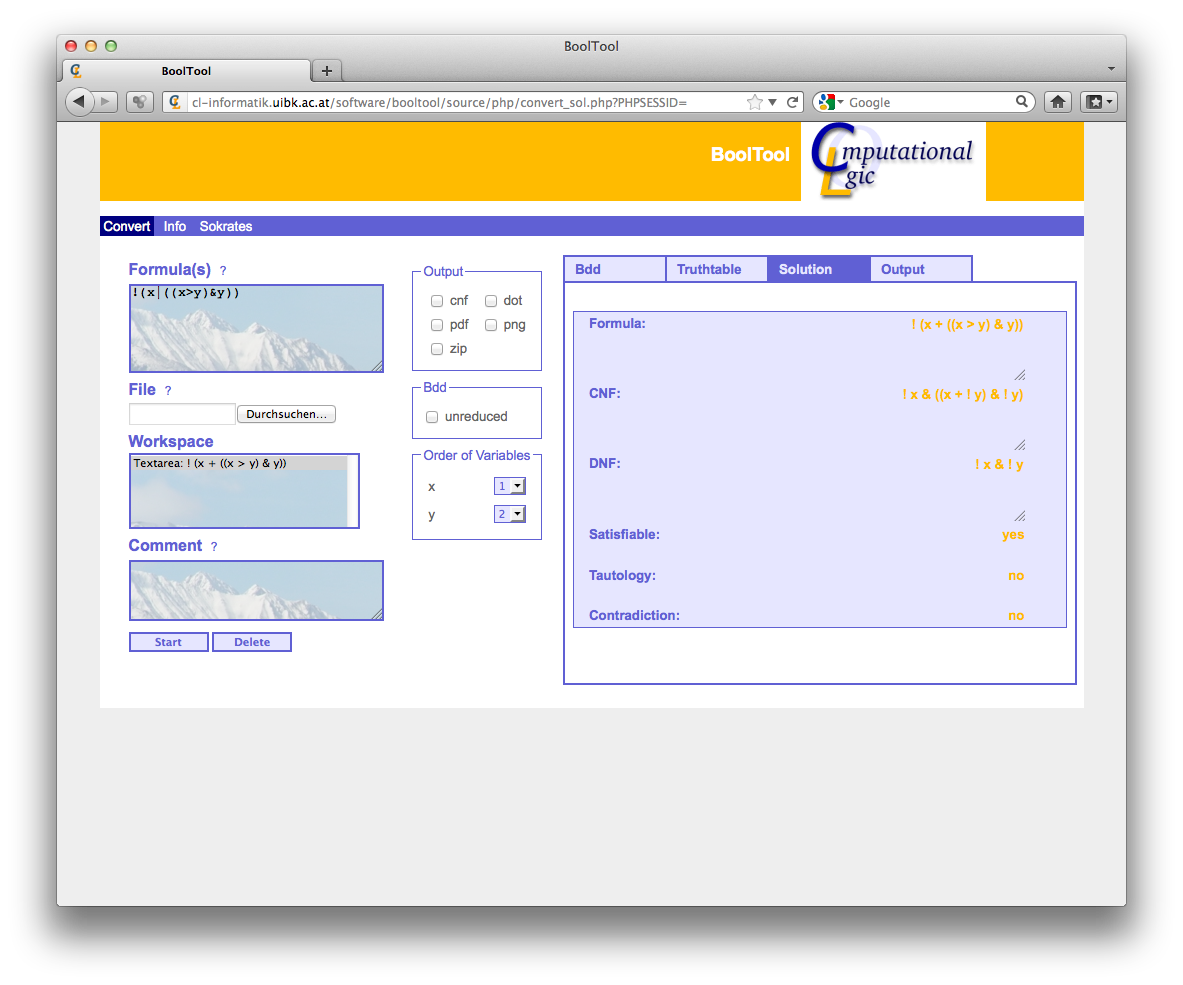
\includegraphics[scale=0.45]{initimgs/BoolToolInterface.png}
%\caption{default}
%\label{default}
%\end{center}
%\end{figure}

}
	
\frame{
	\frametitle{BoolTool}
	\framesubtitle{Drawbacks}
	
	\begin{itemize}
	\item Syntax is slightly different
	\item Semantics is not explained
	\item Normal forms are not defined
	\item Transformations are not demonstrated
	
	\end{itemize}
	
%	\vfill
%	
%	User can not learn many facts about propositional logic.
}

\frame {
	\frametitle{Project Aim}
	\framesubtitle{Allow the user to learn}

	\begin{itemize}
	
	\item Formalism of propositional logic
	
	\item Separation of syntax and semantics
	
	\item Normal forms (NNF, CNF, DNF)

	\item Standard transformations of Boolean functions
	
	\item Coherence of different representations
		
	\end{itemize}

}

%\section{Quellen}

\frame {
	\frametitle{Part I: Design}

	\framesubtitle{Platform agnostic}
	
	\begin{itemize}
	
	\item Self-explanatory environment
	
	\item Glossary of technical terms
	
	\item Tutorials for general concepts and definitions
	
	\item Playgrounds to build and transform formulae
	
\end{itemize}
}

\frame {
	\frametitle{Part II: Implementation}

	\framesubtitle{Platform specific}
	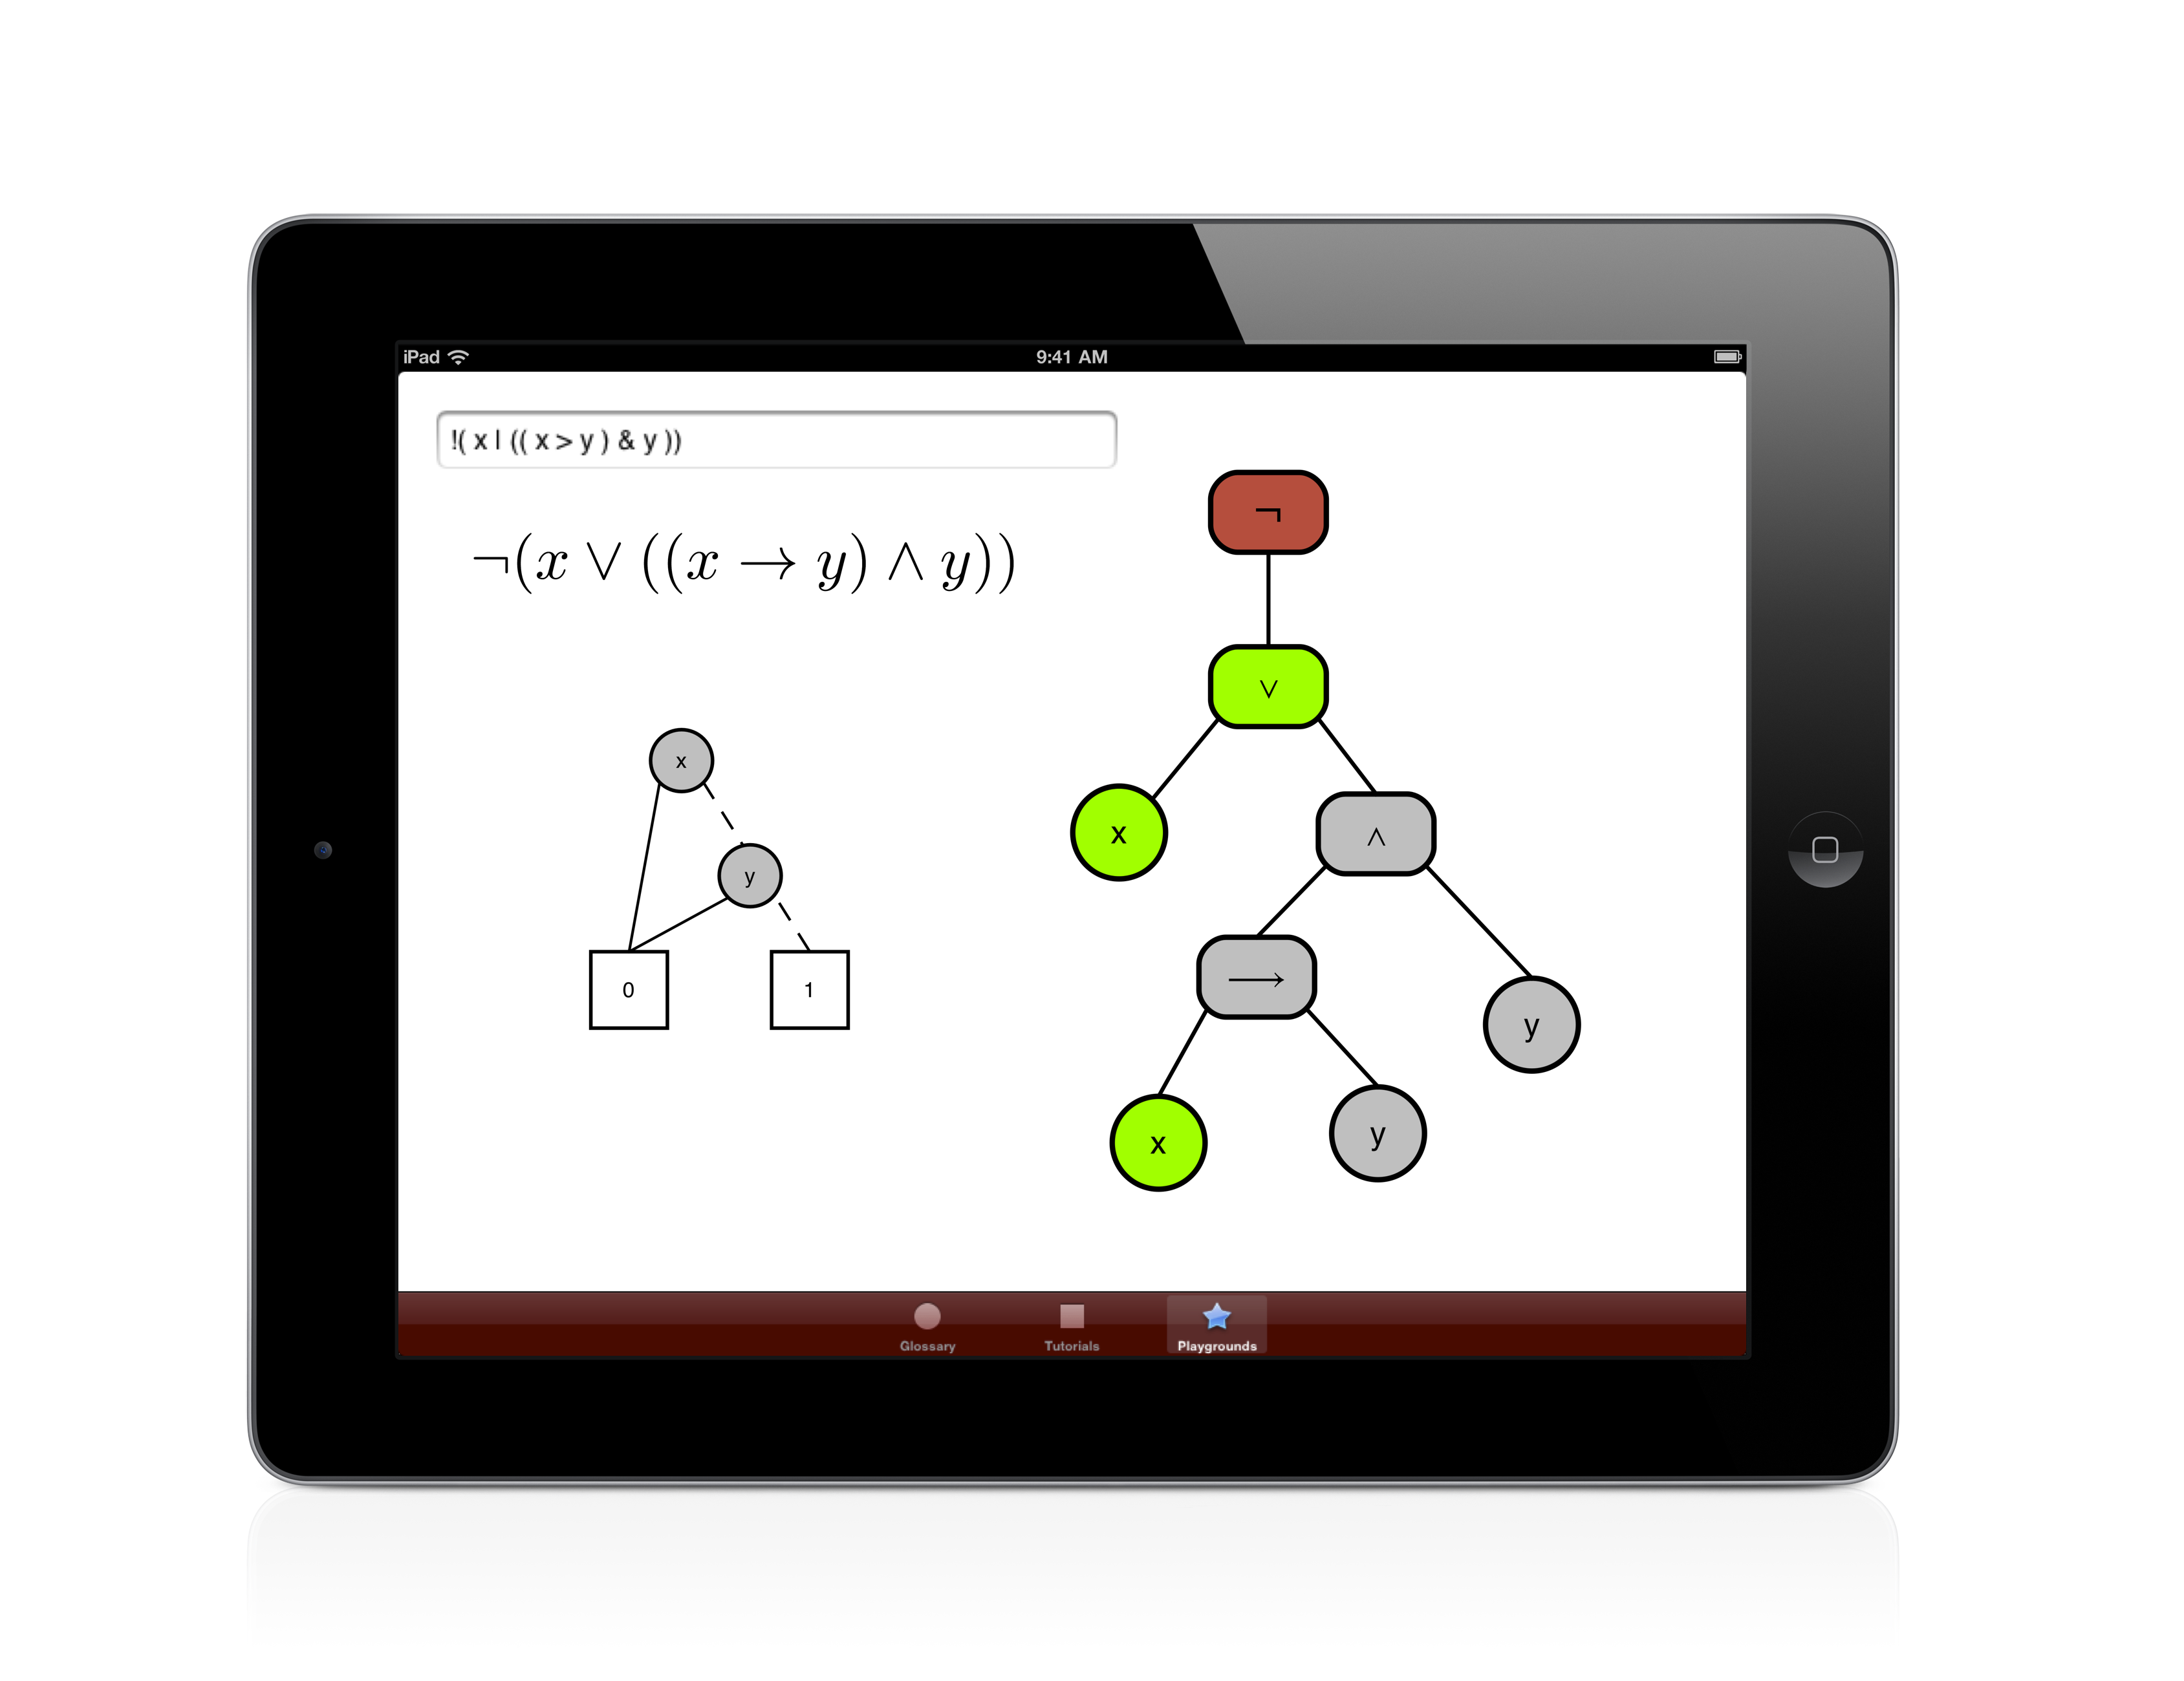
\includegraphics[width=12.2cm,trim=1.5cm 4cm 2cm 2cm]{initimgs/BoolPad6}
}

\section{Sources}
\frame{
	\frametitle{Sources}
	
	\begin{itemize}
	\item Barwise, Etchemendy und Barker Plummer, \textbf{Tarski's World}
	\item Middeldorp, \textbf{Logic}, Lecture 
	\item Huth and Ryan, \textbf{Logic in Computer Science}
	\item OCaml Sourcecode for BoolTool
	\item Scofield, \textbf{Cross Compiling OCaml to iOS} %, \href{http://psellos.com/ocaml/compile-to-iphone.html}{www.psellos.com}
	
	\end{itemize}
}

%\section{Tools}
%\frame{
%	\frametitle{Tools}
%	
%	\begin{itemize}
%	\item XCode
%	\item Objective C
%	\item Cocoa
%	
%		
%	\end{itemize}
%}


\end{document}
